\documentclass[11pt]{article}
\usepackage{times}
\usepackage{ifthen}
\usepackage[dvips]{graphics}
\usepackage[dvips]{color}
\usepackage{epsfig}
%\usepackage{subfigure}
\usepackage[dvips,colorlinks,bookmarks,pdfpagemode=UseOutlines,linkcolor=blue,pagecolor=blue,urlcolor=blue,letterpaper]{hyperref}
\begin{document}
% File giving definitions of commands and environments.
% Because of a latex bug with counters, this has to be included
% using \input not \include.

%--------------------------------------------------------------------------
% For the set of reals and integers
\newcommand{\rr}{\set{Reals}}
\newcommand{\ii}{\set{Integers}}
\newcommand{\cc}{\set{Complex}}
\newcommand{\nn}{\set{Naturals}}

%--------------------------------------------------------------------------
% For figure captions.
% Puts them in sanserif font, indented on both sides.
%   arg: The caption.
\newcommand{\figcaption}[1]{\textsf{\begin{center}\begin{minipage}{5in}
\caption{#1}
\end{minipage}\end{center}}}

%--------------------------------------------------------------------------
% For terms being defined.
% Puts them in bold face and creates an index entry.
%   arg: The term being defined.
% NOTE: To get boldface in the index, do |textbf after #1.
% But this breaks hyperlinks.
\newcommand{\defn}[1]{\textbf{#1}\index{#1}}

%--------------------------------------------------------------------------
% For terms being indexed.
% Puts them in standard font face and creates an index entry.
%   arg: The term being defined.
\newcommand{\pointer}[1]{#1\index{#1}}

%--------------------------------------------------------------------------
% For bold terms to be index, but defined elsewhere
% Puts them in bold face and creates an index entry.
%   arg: The term being defined.
\newcommand{\strong}[1]{\textbf{#1}\index{#1}}

%--------------------------------------------------------------------------
% For terms to be index, but defined elsewhere
% Puts them in normal face and creates an index entry.
%   arg: The term being defined.
\newcommand{\idx}[1]{#1\index{#1}}

%--------------------------------------------------------------------------
% For set names.
% Puts them in italics. In math mode, yields decent spacing.
%   arg: The name of the set.
\newcommand{\set}[1]{\mbox{\textit{#1}}}

%--------------------------------------------------------------------------
% For real part.
%   arg: The argument of the real part.
\newcommand{\re}[1]{\mbox{\textit{Re}}\{#1\}}

%--------------------------------------------------------------------------
% For imaginary part.
%   arg: The argument of the imaginary part.
\newcommand{\im}[1]{\mbox{\textit{Im}}\{#1\}}

%--------------------------------------------------------------------------
% For matlab commands
%   arg: The name of the command
\newcommand{\matlab}[1]{\texttt{#1}\index{#1 command in Matlab}\index{Matlab!#1}}
\newcommand{\simulink}[1]{\texttt{#1}\index{#1 in Simulink}\index{Simulink!#1}}
\newcommand{\matlabInCaption}[1]{\texttt{#1}}

%--------------------------------------------------------------------------
% For "Probing Further" sidebars.
% Puts them in a floating frame.  It is up to you to ensure that the
% frame fits on one page.
%   arg: the title.
\newenvironment{further}[1]{
\begin{table}[btp]
\centering
\begin{tabular}{|p{5in}|}
\hline
\cr
\begin{minipage} {5in}
\parskip        0.1in
\parindent      0.0in
\subsection* {Probing further: #1}
\addcontentsline{toc}{subsection}{Probing further: #1}
} {
\end{minipage}\cr
\cr
\hline
\end{tabular}
\end{table}
}

%--------------------------------------------------------------------------
% For "Basics" sidebars.
% Puts them in a floating frame.  It is up to you to ensure that the
% frame fits on one page.
%   arg: the title.
\newenvironment{basics}[1]{
\begin{table}[btp]
\centering
\begin{tabular}{|p{5in}|}
\hline
\cr
\begin{minipage} {5in}
\parskip        0.1in
\parindent      0.0in
\subsection* {Basics: #1}
\addcontentsline{toc}{subsection}{Basics: #1}
} {
\end{minipage}\cr
\cr
\hline
\end{tabular}
\end{table}
}

%--------------------------------------------------------------------------
% For "Tips and Tricks" sidebars.
% Puts them in a floating frame.  It is up to you to ensure that the
% frame fits on one page.
%   arg: the title.
\newenvironment{tricks}[1]{
\begin{table}[btp]
\centering
\begin{tabular}{|p{5in}|}
\hline
\cr
\begin{minipage} {5in}
\parskip        0.1in
\parindent      0.0in
\subsection* {Tips and Tricks: #1}
\addcontentsline{toc}{subsection}{Tips and Tricks: #1}
} {
\end{minipage}\cr
\cr
\hline
\end{tabular}
\end{table}
}

%--------------------------------------------------------------------------
% For text that is boxed for emphasis.
\newenvironment{boxed}{
\begin{center}
\begin{tabular}{|p{5in}|}
\hline
\cr
\begin{minipage} {5in}
\parskip        0.1in
\parindent      0.0in
} {
\end{minipage}\cr
\cr
\hline
\end{tabular}
\end{center}
}

%--------------------------------------------------------------------------
% For examples
% NOTE: Because of this line, this has to be included using \input
% not \include.
\newcounter{example}
\newenvironment{example}{
\refstepcounter{example}
\begin{quote}
\textbf{Example \arabic{chapter}.\arabic{example}:}
} {
\end{quote}
}
\renewcommand \theexample {\thechapter.\arabic{example}}


\title{Two-Dimensional Technical Specification for Soft Walls}
\author{J. Adam Cataldo, Edward A. Lee, and
Xiaojun Liu\\ \{acataldo, eal, liuxj\}@eecs.berkeley.edu\\ Electrical
Engineering \& Computer Science\\ University of California, Berkeley\\
\\} 
\date{13 April 2002}

\maketitle

%-----------------------------------------------------------------------------
%-----------------------------------------------------------------------------

\section{Introduction}

The terrorist attacks of September 11, 2001 proved that airplanes make
deadly bombs.  In response to this attack-by-aircraft threat, Edward
Lee proposed \textit{soft walls}, a flight control system that
prevents aircrafts from entering \textit{no-fly zones}, that is,
restricted airspace, such as major cities, government centers,
military installations, chemical factories, and nuclear-power plants
\cite{Lee}.  The major objective of this control scheme is to minimize
the control imposed on pilots while protecting the no-fly zones.  This
control scheme uses a map from the aircraft's database together with
position, velocity, and orientation information from onboard sensors
to prevent no-fly zone entry.

This document describes our first approach at a softwalls control
algorithm.  We assume the aircraft travels in a horizontal plane at a
constant velocity and can only turn as control.  The no-fly zone is
bounded by a line in the 2D plane.  While these approximations are
unrealistic, we chose a simple model, which we will later refine for
accuracy.

%-----------------------------------------------------------------------------
%-----------------------------------------------------------------------------


\section{Two-Dimensional Model}

%-----------------------------------------------------------------------------


\subsection{Two-Dimensional Aircraft Model}

In our two-dimensional model we only control the aircraft's heading.
Let the aircraft's position be a function
\[
p \colon \rr \to \rr \times \rr
\]
where the domain is time (the reals) and the range is the aircraft's
two-dimensional position.  Let $\dot{p}$ denote the time derivative
(the velocity) and $\ddot{p}$ the second derivative with respect to
time (the acceleration). Let $p_x$ denote the $x$-direction position
(east-west, increasing to the east) and $p_y$ the $y$-direction
position (north-south, increasing to the north). Similarly,
$\dot{p_x}$ and $\ddot{p_x}$ denote the $x$-direction speed and
acceleration.

Let the aircraft's speed $s$ be given by
\[
\forall ~ t \in \rr, \quad
s(t) = |\dot{p}(t)| .
\]
Let
\[
\theta \colon \rr \to [-\pi, \pi)
\]
be the aircraft's heading, where $0$ is due east, so that
\[
\forall ~ t \in \rr, \quad
\dot{p} (t) = (s(t) \cos(\theta (t)), s(t) \sin(\theta(t))) .
\]

Assume that during flight, the pilot controls the heading's rate of
change, $\dot{\theta}$, with differential thrust and movement of the
rudder, ailerons, and elevator.  Moreover, the pilot controls the
speed via overall thrust and vertical movement.  In this model, which
we show in figure \ref{fig2Daircraft}, the the aircraft-model's inputs
are $\dot{\theta}$ and $s$.

\begin{figure}[btp]
\centering
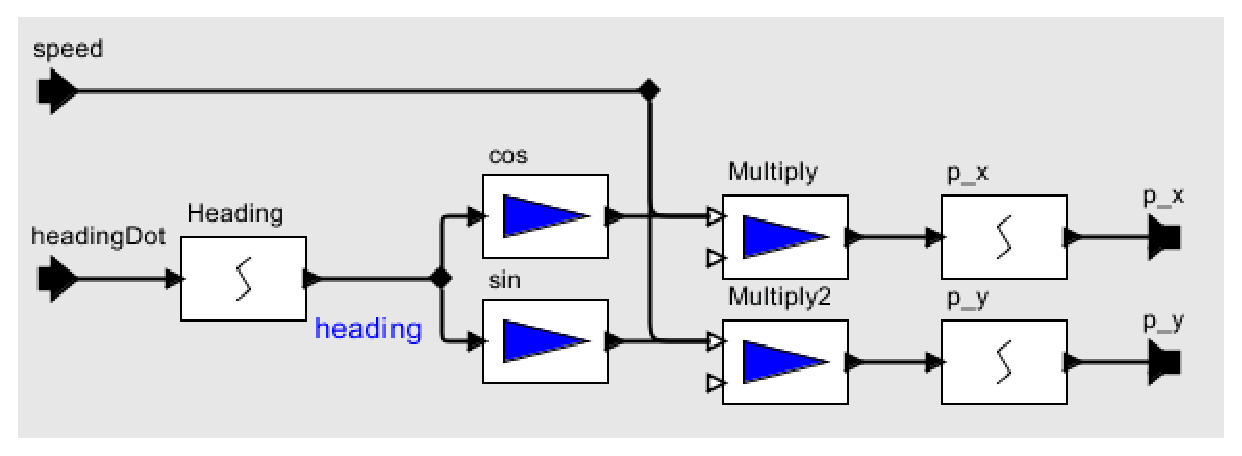
\includegraphics[width=5in]{fig2Daircraft.eps}
\figcaption{Two dimensional aircraft model.
\label{fig2Daircraft}}
\end{figure}

%-----------------------------------------------------------------------------

\subsection{Turn Radius}

Assume the speed is a constant $s$, with $s$ given in meters per
second, so the pilot controls only heading.  If the heading's rate of
change is a constant, $\dot{\theta} = \alpha$, with $\alpha$ given in
radians/second, it takes $\tau = 2 \pi /\alpha$ seconds to complete
one circle.  Upon completing the circle, the aircraft has covered a
$s\tau = 2 \pi s/\alpha$ meter distance.  Since the circle's radius
times $2 \pi$ gives its circumference, the turning radius is
\[
r = s/\dot{\theta} .
\]

Thus, the heading's rate of change is
\[
\dot{\theta} = s/r.
\]
If we know minimum-safe-turning radius is $r_{min}$, then the control
signal $\dot{\theta}$ must be kept in the range $[-s/r_{min},
s/r_{min}]$.

For example, an aircraft traveling at
\[
s = 500~ kilometers/hour
\]
(139 meters/second) with a minimum safe turning radius $r_{min} =
1000$ meters constrains the pilot's safe $\dot{\theta}$ to the range
$[-0.139, 0.139]$ radians per second.

%-----------------------------------------------------------------------------

\subsection{Blending Controller}

Let the pilot's control signal be $\dot{\theta}_p$ and the
softwalls-generated control signal be $\dot{\theta}_s$.  We take the
aircraft heading's rate of change to be
\[
\dot{\theta} = \set{limit}_{[-s/r_{min}, s/r_{min}]}
(\dot{\theta}_p - \dot{\theta}_s ),
\]
where $\set{limit}_{[a,b]}$ is a function
\[
\set{limit}_{[a,b]} \colon \rr \to [a, b]
\]
where
\[
\forall ~ u \in \rr, \quad
\set{limit}_{[a,b]}(u) = \left \{
\begin{array}{ll}
b&\mbox{ if } u > b,\\
a&\mbox{ if } u < a,\\
u&\mbox{ otherwise. }
\end{array}
\right .
\]
This strategy blends the softwalls and pilot control signals ensuring
that while the control parameter is within safe limits, the aircraft's
response to the pilot's control signal remains unattenuated.

%-----------------------------------------------------------------------------

\subsection{Maintaining Responsiveness}

\begin{figure}[btp]
\centering
\includegraphics{bias.eps}
\figcaption{Rate of change of heading vs. pilot-specified rate of
change of heading.  Here a left turn is on the right side of the
graph because a positive $d\theta/dt$ will cause the plane to turn
left.
\label{figBias}}
\end{figure}

Figure \ref{figBias} illustrates the blending controller maintaining
responsivity while biasing the pilot control.  When the softwalls
controller adds no bias, the aircraft will turn as the pilot
intends. That is, the actual $\dot{\theta}$ equals the pilot's
$\dot{\theta}_{p}$.  Suppose the softwalls bias is $-M = -s/r_{min}$,
where $M$ is the maximum rate of change in heading.  The bias is
rightward, and the pilot will be unable to turn the aircraft left, and
if the pilot attempts to turn left at the maximum rate $M$, the
aircraft will keep straight.  When the bias increases to $-3M/2$, also
rightward, the aircraft will turn right at a rate greater than or
equal to $-M/2$ for any pilot control signal.

With this scheme, a cooperative pilot will turn away from the soft
wall to reduce the bias.  An uncooperative pilot, however, will
attempt a turn towards the wall even with the bias applied.  When the
bias exceeds $-M$, this pilot will be unable to overcome the bias, and
with the controls saturated, the aircraft will turn away from the soft
wall.

Until the actual $\dot{\theta}$ saturates, the aircraft responds
exactly as the pilot expects.  That is, when the response curve's slope (figure
\ref{figBias}) is not zero, it is one.

%-----------------------------------------------------------------------------
%-----------------------------------------------------------------------------

\section{Criticality-Based Control}

To asses an aircraft's threat to a no-fly zone, we created a
criticallity measurement.  From this we compute the bias, $\theta_s$,
if any.

%-----------------------------------------------------------------------------

\subsection{A Measure of Criticality}

\begin{figure}[btp]
\centering
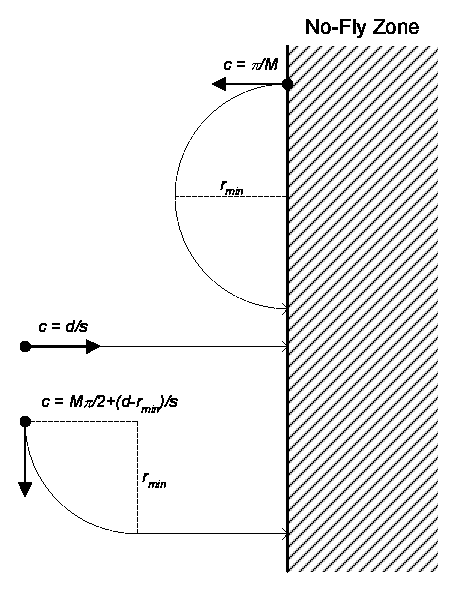
\includegraphics{criticality.eps}
\figcaption{Calculating $T(x,\,\theta)$ for criticality measure.
\label{figCriticality}}
\end{figure}

Our criticality measurement is inversely proportional to the minimum
time it takes the aircraft to enter the no-fly zone.  Figure
\ref{figCriticality} illustrates this measure.  In this figure, the
black dots represent the aircraft's position, and the arrows represent
its heading. For each position and heading, we plot the worst-case
trajectory, i.e., the path that takes the aircraft into the
no-fly zone faster than all other paths, as dotted lines.  In this
sense, we are calculating an optimal path for the plane to collide with
the no-fly zone.

Suppose we define the no-fly zone as the regioin $\{(x,y)|\ x \geq b_{x}\}$. Then the
criticality measurement, $c$, and the aircraft's $y$-position are
independent. We let  $c(x, \theta) = 1 / T(x, \theta)$ where
$T(x, \theta)$, the minimum time a plane needs to contact the no-fly
zone, comes from
\begin{equation}
T(x, \theta) = \left\{ \begin{array}{ll}
\frac{\theta}{M} + \frac{d - r_{min}\sin{\theta}}{s} & \mbox{if $d \geq r_{min}\sin{\theta},\ 0 \leq \theta \leq \pi/2$} \\
\frac{\theta - \arcsin{\left( \frac{r_{min}\sin{\theta}- d}{r_{min}}\right) }}{M} & \mbox{if $d < r_{min}\sin{\theta},\ 0 \leq \theta \leq \pi/2$} \\
\frac{2(\theta - \pi/2)}{M} + T(x, \pi - \theta) & \mbox{if $\pi/2 < \theta \leq \pi$} \\
T(x, |\theta|) & \mbox{if $-\pi \leq \theta < 0$}
\end{array}
\right. \label{eq:bigT}
\end{equation}
where $d = b_{x} - x$ is the distance between the aircraft and the no-fly zone.
Note that $s$, $r_{min}$, and $M$ are related by $M = s/r_{min}$.

Note that if the aircraft is at the wall and heading directly away
from it, as in the top diagram of figure \ref{figCriticality}, then
the minimum time for aircraft/no-fly zone collision is the time
required to traverse a semi-circle with radius $r_{min}$.  This is
$\pi/M$.  If the aircraft is at distance $d$ from the wall and heading
straight towards it, then the minimum time to contact is $d/s$, where
$s$ is the (fixed) speed.  If the aircraft is at distance $d$ from the
wall (greater than $r_{min}$) but heading parallel to it, then the
time it will take to reach the wall is
\[
T = \pi M/2+(d-r_{min})/s .
\]

%-----------------------------------------------------------------------------

\subsection{Criticality-Based Soft Wall Controller}

\begin{figure}[btp]
\centering
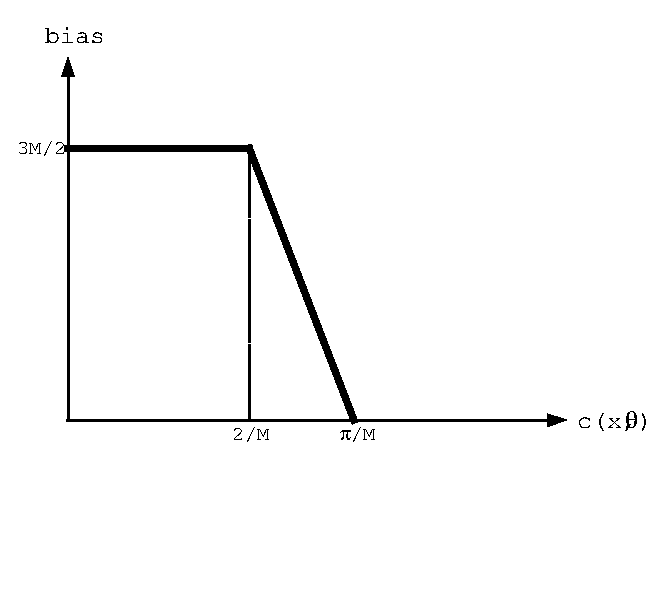
\includegraphics{criticalityBias.eps}
\figcaption{Bias as a function of criticality.
\label{figCriticalityBias}}
\end{figure}

The proposed criticality-based controller produces the bias shown in
figure \ref{figCriticalityBias}.  The threshold $M/\pi$ is the value
of $c(x, \theta)$ when $x = b_{x}$ (the aircraft is on the boundary of
the no-fly zone), and $\theta = \pi$ (the aircraft is flying straight
out of the no-fly zone). No bias is needed here, nor for smaller
criticality.  The threshold $M/2$ is equal to $c(b_{x}-2r_{min}, 0)$
-- the aircraft is flying straight towards the no-fly zone at a
distance of $2r_{min}$ from the zone.  The aircraft can still safely
turn away at half the maximum turning rate. Note that the maximum bias
level is at $3M/2$, so the plane will be turned at a rate of at least
half the maximum, irrespective of pilot input. The bias sign convention
is the same as $\theta$ (positive -- left, negative -- right).

%-----------------------------------------------------------------------------

\subsection{Simulation Results}

\begin{figure}[btp]
\centering
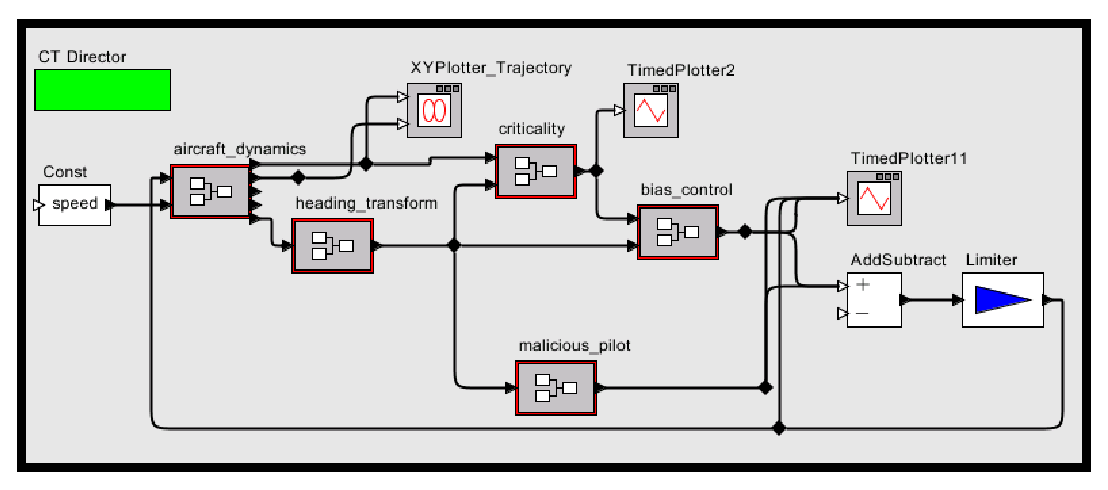
\includegraphics[width=5in]{criticalityTopLevel.eps}
\figcaption{Top-level of a model with a maximally uncooperative pilot.
\label{figCriticalityTopLevel}}
\end{figure}

\begin{figure}[btp]
\centering
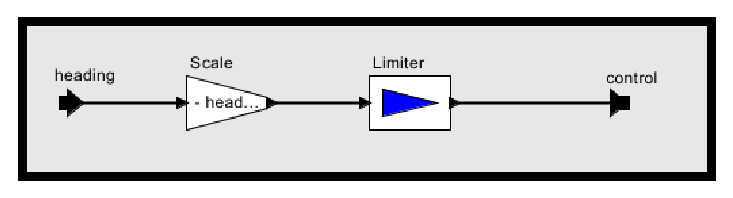
\includegraphics{maliciousPilot.eps}
\figcaption{Maximally uncooperative pilot model.  The scale factor is large.
\label{figMaliciousPilot}}
\end{figure}

\begin{figure}[btp]
\centering
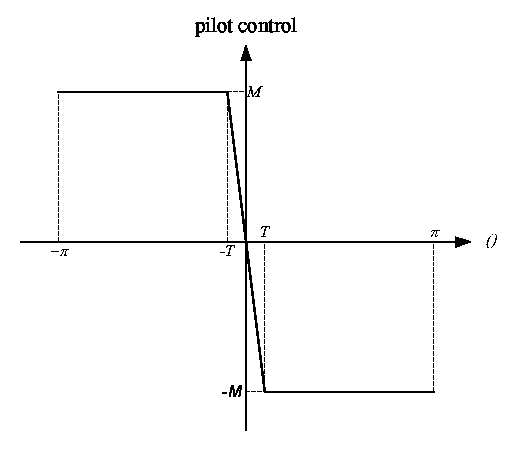
\includegraphics{pilotControl.eps}
\figcaption{Pilot control as a function of heading for the maximally
uncooperative pilot.
\label{figPilotControl}}
\end{figure}

We constructed the model of figure \ref{figCriticalityTopLevel} with
Ptolemy II to simulate the proposed controller. The \emph{aircraft
dynamics} component contains the aircraft model of figure
\ref{fig2Daircraft}. The \emph{malicious pilot} component implements
the control strategy of figure \ref{figMaliciousPilot}. Here, the
pilot tries to fly the aircraft into the no-fly zone by maintaining
the heading $\theta$ at 0. This is accomplished by multiplying the
heading by a large number and limiting the result to a number in the
safe-control range.  Intuitively, the pilot will attempt to turn
maximally towards the wall whenever the current heading deviates from
the heading directly towards the wall, as shown in figure
\ref{figPilotControl}.  When the plane is approaching the wall, this
pilot does not try to turn.  The nonzero slope near $\theta = 0$
prevents the system from exhibiting Zeno behavior.  The
\emph{criticality} component calculates $c(x, \theta)$. The \emph{bias
control} component implements the soft wall controller. The output
from the pilot and the controller are combined and limited to the
range $[-M, M]$ before fed back to the aircraft model.

\begin{figure}[btp]
\centering
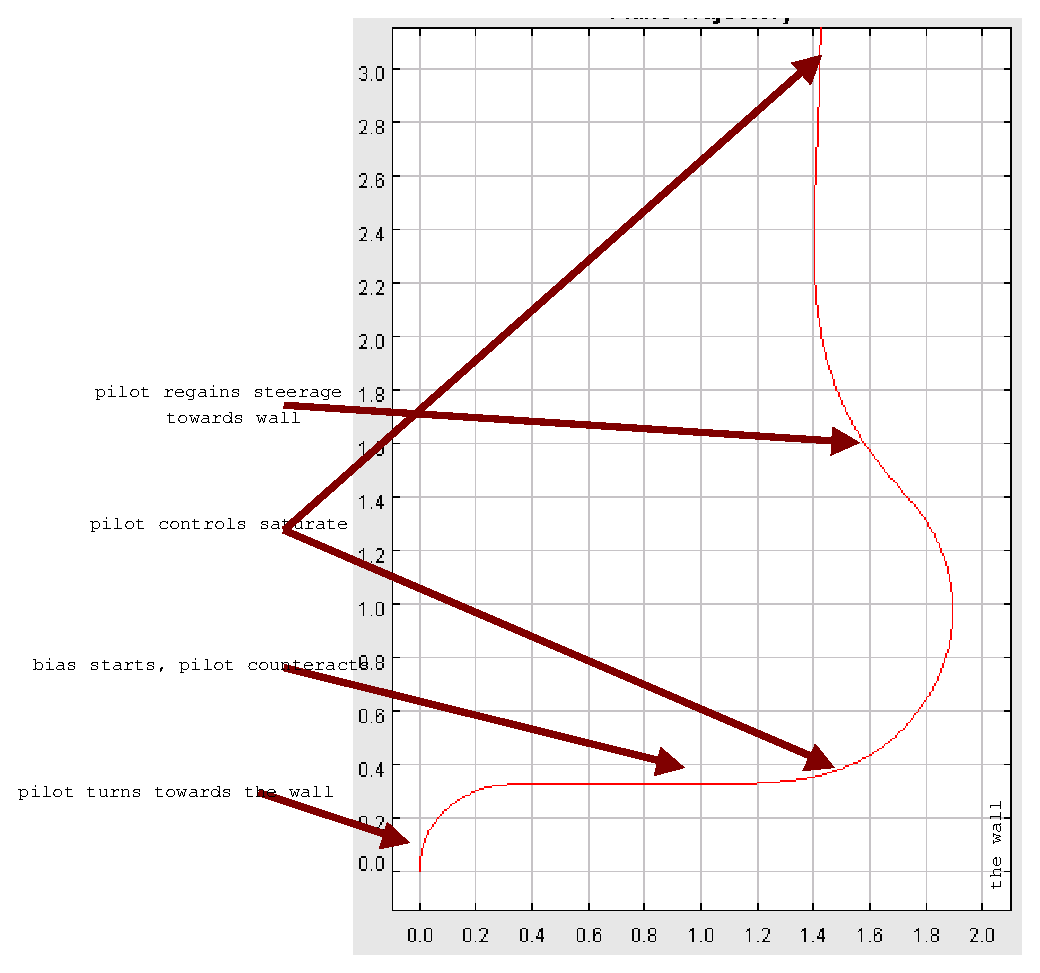
\includegraphics[width=5in]{simulationRun.eps}
\figcaption{Simulation run with a maximally
uncooperative pilot.
\label{figSimulationRun}}
\end{figure}

Figure \ref{figSimulationRun} shows a simulation run.  In our
simulation the aircraft initially flies parallel to the no-fly zone
($\theta = \pi / 2$), at a distance of 2 miles. The speed of the
aircraft is a constant 360 miles per hour. The maximum turning rate is
$2\pi/20$, so that the aircraft can complete a circle in 20
seconds. (Note that these numbers are fictional. Later simulations
will use real aircraft-performance characteristics.)

The aircraft starts at the lower left, traveling upwards, and the
no-fly zone is two miles to the right, with its boundary oriented
vertically.  Initially, the malicious pilot freely turns the aircraft
toward the no-fly zone. When the aircraft is within 1 mile from the
zone, the controller starts biasing the pilot control. Before the bias
control reaches $M$, the pilot mitigates the bias and keeps the
aircraft heading toward the no-fly zone, but the pilot control finally
saturates when $\theta_{s} = M$, and the soft wall controller turns
the aircraft around at half the maximum rate. As the criticality
decreases, the bias from the controller becomes smaller. The pilot
regains steerage towards the no-fly zone, but the aircraft settles in
flying parallel to the zone. At this time, the pilot is still trying
in vain to fly the aircraft into the no-fly zone by placing the
control at the right maximum.

We are still improving this criticality-based control scheme. At
present, we are simulating a variety of flight scenarios, and
investigating interactive simulation where experimenters control the
pilot's output.

%-----------------------------------------------------------------------------

\subsection{Criticality-Based Control Verification}

\subsubsection{Validity of the Criticality Measure}

The trajectories we use to calculate $T(x,\ \theta)$ are illustrated in
figure~\ref{figCriticality}. Such trajectories are achieved by first turning
the aircraft toward flying straight on to the no-fly zone at the maximum
rate $M$, then maintaining that direction. In the following we argue that
such trajectories indeed yield the shortest time to reach the no-fly zone.

Let $\dot{x}(t)$ denote the plane's velocity in the direction
perpendicular to the wall, and let $\theta(t)$ denote the plane's
heading.  From our aircraft model, where $s$ is the plane's constant
speed,
\[
\dot{x}(t) = s \cos{(\int_{0}^{t}{\dot{\theta}}(\hat{t})d\hat{t})}
\]
Here $\dot{\theta}(t)$ is the heading's rate of change.  When the
softwalls system applies no bias, this signal equals the pilot input.
$\theta$ is always in the range $[-s / r_{min}, s / r_{min}]$.

When $x(t) < b_{x}$, i.e., the plane is left of the no-fly zone, the
plane approaches the no-fly zone faster as $\dot{x}(t)$ increases.
The maximum value of $\dot{x}(t)$ is $s$.  If $\theta(t) = 0$, then
$\dot{x}(t) = s$, so an input of $\dot{\theta}(t) = 0$ will cause the
plane to move to the wall the fastest.  When $\theta(t) \neq 0$, as
$\theta(t) \rightarrow 0, \dot{x}(t) \rightarrow s$.  For $\theta(t)
\in (0,\pi]$, the fastest way to make $x(t) \rightarrow s$ is to set
$\dot{\theta}(t) = -M$, where $M$ is the maximum turning rate.  In
this range of angles, $\dot{x}(t)$ will be strictly increasing at the
maximum rate, so this is the fastest approach to the wall.  Similarly,
when $\theta(t) \in (-\pi, 0)$, the fastest approach to the wall uses
$\dot{\theta}(t) = M$ until $\theta(t) = 0$.  The criticality measure
uses this strategy to calculate the minimum time for aircraft/no-fly
zone collision, so it is a valid minimum-time calculation.

\subsubsection{Safety of Criticality-Based Control}

We assume that the initial position of the aircraft is at least $2r_{min}$ from
the no-fly zone. With the criticality-based control strategy discussed earlier
in this section, we show that the aircraft cannot be flown into the
no-fly zone, no matter what the pilot does.

At the initial position, the criticality $c \leq M/\,2$. Because $c$ is a
continuous function of $x$ and $\theta$, along any potential trajectory from
the initial position to the no-fly zone, there must be a point where
$c(x,\ \theta) = M/\,2$. The pair $x,\ \theta$ satisfying this equation is
related by
\[x = 
\left\{ \begin{array}{ll}
b_x - r_{min}(2 + \sin\!|\,\theta| - |\,\theta|) & |\,\theta| \leq 2 
\\
b_x - r_{min}(\sin\!|\,\theta| - \sin(|\,\theta|-2)) & 2 < |\,\theta| \leq \pi/\,2 + 1
\end{array}
\right.
\]
$c(x,\ \theta)$ is always less than $M/\,2$ when $|\,\theta| > \pi/\,2 + 1$.

If a malicious pilot wants to fly the aircraft from a point where 
$c(x,\ \theta) = M/\,2$ into the no-fly zone, the pilot has to prevent the
criticality from decreasing to a value less than $M/\,2$. Given the bias added
by our control strategy, the aircraft will be turned away from the no-fly zone
at a minimum rate of $M/\,2$ when $c(x,\ \theta) \geq M/\,2$. Starting at a
point where $c(x,\ \theta) = M/\,2$, the maximum $x$-coordinate that the
aircraft can reach is given by
\[x_{max} = 
\left\{ \begin{array}{ll}
d_{x} - r_{min}(3\sin\!|\,\theta| - |\,\theta|) & |\,\theta| \leq \pi/\,2
\\
d_{x} - r_{min}(2 + \sin\!|\,\theta| - |\,\theta|) & \pi/\,2 < |\,\theta| \leq 2
\\
d_{x} - r_{min}(\sin\!|\,\theta| - \sin(|\,\theta|-2)) & 2 < |\,\theta| \leq \pi/\,2 + 1
\end{array}
\right.
\]
$x_{max}$ is never greater than $b_x$, so the aircraft is never inside the
no-fly zone.

%-----------------------------------------------------------------------------
%-----------------------------------------------------------------------------

\section{Summary}

We have described a simple control algorithm to keep an aircraft out
of a no-fly zone with a straight-line boundary in two dimensions.  Our
strategy maintains maximal responsiveness to pilot controls subject to
the constraint that we forbid no-fly zone entry.

\begin{thebibliography}{Lee 2001}

\bibitem[Lee 2001]{Lee}
Edward A. Lee.  ``Soft Walls - Modifying Flight Control Systems to
Limit the Flight Space of Commercial Aircraft''.  \textit{Technical
Memorandum UCB/ERL M01/31}.  15 September 2001.

\end{thebibliography}

\end{document}

